\documentclass[12pt, a4paper]{article}

% ===== 패키지 =====
\usepackage{fontspec}         % XeLaTeX/LuaLaTeX 폰트 설정
\usepackage{kotex}            % 한글 지원
\usepackage{geometry}
\geometry{margin=2.5cm}
\usepackage{minted}           % 코드 삽입 (XeLaTeX + shell-escape 필요)
\usepackage{xcolor}           % 색상
\usepackage{booktabs}         % 깔끔한 표
\usepackage{amsmath, amssymb} % 수식
\usepackage{hyperref}         % 하이퍼링크
\usepackage{graphicx}         % 이미지
\usepackage{enumitem}         % 리스트 커스텀
\usepackage{caption}
\usepackage{adjustbox}        % 큰 표 너비 조절용
\usepackage{pifont}           % 체크마크 기호용
\newcommand{\cmark}{\ding{51}}
\usepackage{tikz}             % 순서도 도형
\usetikzlibrary{shapes.geometric, arrows.meta, positioning}

% ===== 코드 스타일 =====
\setminted[python]{
    bgcolor=black!5,
    linenos=true,
    breaklines=true,
    fontsize=\small,
    frame=lines,
    framesep=2mm
}
\setminted[bash]{
    bgcolor=black!5,
    linenos=false,
    breaklines=true,
    fontsize=\small,
    frame=lines,
    framesep=2mm
}

% ========================================
\begin{document}

% ===== 커스텀 헤더 (제목 페이지 없이 바로 시작) =====
\begin{center}
    {\Large\bfseries Programming Assignment \#2}\\[0.4em]
    {\large\bfseries 의사결정 나무(Decision Tree)를 이용한 범주형 데이터 분류기}\\[1em]
    {\normalsize
        \textbf{과목:} Data Science (ITE4005) \quad
        \textbf{학번:} 2023036299 \quad
        \textbf{이름:} 김진욱 \quad
        \textbf{2026.04.03}\\[0.3em]
        \textbf{OS:} Windows 10/11 \quad
        \textbf{Python:} 3.12.10 \quad
        \textbf{라이브러리:} 표준 라이브러리 (\texttt{sys}, \texttt{math}, \texttt{collections})
    }
\end{center}
\vspace{0.5em}
\hrule
\vspace{1em}

% ============================================================
\section{알고리즘 요약}
% ============================================================

\subsection{의사결정 나무 알고리즘 개요}

의사결정 나무(Decision Tree)는 데이터를 속성(Attribute)의 값에 따라 재귀적으로 분할하여 트리 구조의 분류 모델을 학습하는 알고리즘이다. 각 내부 노드에서는 \textbf{정보 이득(Information Gain)}이 가장 높은 속성을 선택해 데이터를 분기하며, 모든 데이터의 클래스가 동일하거나 더 이상 분할할 속성이 없을 때 리프 노드(예측 라벨)를 생성하고 재귀를 종료한다. 본 구현은 모든 속성을 \textbf{범주형(Categorical)}으로 취급하여 N-갈래 분기를 수행하며, 동점(Tie) 상황에서 \textbf{Gain Ratio}를 보조 기준으로 사용하는 혼합(Hybrid) 전략을 채택하였다.

\subsection{전체 순서도}

\begin{figure}[h]
\centering
\begin{tikzpicture}[
    node distance=0.75cm and 2cm,
    box/.style={rectangle, rounded corners=5pt, draw=black!70, fill=blue!8,
                minimum width=9cm, minimum height=0.8cm,
                align=center, font=\small},
    loopbox/.style={rectangle, rounded corners=5pt, draw=black!60, fill=orange!10,
                    minimum width=9cm, minimum height=1.6cm,
                    align=center, font=\small},
    arr/.style={->, thick, draw=black!60}
]
\node[box]      (start)  {시작};
\node[box, below=of start]    (read)   {\texttt{read\_data()} \\ 학습 데이터 / 테스트 데이터 파싱};
\node[box, below=of read]     (split)  {\texttt{header[-1]} = target \quad \texttt{header[:-1]} = features \\ 타겟(정답열) / 피처(재료열) 분리};
\node[loopbox, below=of split] (build) {
    \texttt{build\_tree()} $\leftarrow$ 재귀 호출 \\
    \texttt{select\_best\_attribute()} \\
    \texttt{information\_gain()} + \texttt{entropy()} $\leftarrow$ 1차 기준 \\
    \texttt{gain\_ratio()} + \texttt{split\_info()} $\leftarrow$ 동점 시 보조 기준
};
\node[box, below=of build]    (pred)   {\texttt{predict\_all()} $\to$ \texttt{predict\_one()} $\leftarrow$ 재귀 호출 \\ 테스트 데이터 예측};
\node[box, below=of pred]     (write)  {\texttt{write\_result()} \\ 결과 파일 저장};
\node[box, below=of write]    (end)    {종료};

\draw[arr] (start) -- (read);
\draw[arr] (read)  -- (split);
\draw[arr] (split) -- (build);
\draw[arr] (build) -- (pred);
\draw[arr] (pred)  -- (write);
\draw[arr] (write) -- (end);
\end{tikzpicture}
\caption{의사결정 나무 분류기 전체 파이프라인}
\end{figure}

\subsection{핵심 자료 흐름}

\begin{verbatim}
read_data -> list[dict] -> build_tree -> nested dict (트리)
                                           |
                        predict_all -> list[str] (예측 라벨)
                                           |
                        write_result -> result file (탭 구분 텍스트)
\end{verbatim}

트리는 \textbf{중첩 딕셔너리} (\texttt{\{속성명: \{속성값: 서브트리, ...\}\}})로 표현되며, 리프 노드는 예측 라벨 \textbf{문자열(str)}로 저장된다. 데이터의 각 행은 \texttt{\{속성이름: 값\}} 형태의 \textbf{딕셔너리}로 파싱되어, 코드 전체에서 인덱스 번호 없이 속성 이름으로 값에 접근한다.


% ============================================================
\section{각 함수별 코드 상세 설명}
% ============================================================

% --- 2.1 ---
\subsection{\texttt{read\_data(file\_path)} --- 데이터 파싱}

탭(\texttt{\textbackslash t})으로 구분된 데이터 파일을 읽어 헤더와 데이터 리스트로 변환한다.

\begin{minted}{python}
header = lines[0].strip().split('\t')
data = []
for line in lines[1:]:
    line = line.strip()
    if not line:
        continue
    values = line.split('\t')
    row = dict(zip(header, values))
    data.append(row)
return header, data
\end{minted}

\noindent\textbf{핵심 설계 결정:}
\begin{itemize}
    \item \textbf{\texttt{dict(zip(header, values))} 채택}: 각 행을 \texttt{\{속성이름: 값\}} 딕셔너리로 변환한다. 이를 통해 코드 전체에서 \texttt{row['age']}, \texttt{row['buying']} 처럼 속성 ``이름''으로 값에 접근할 수 있다. 인덱스 번호(\texttt{row[0]}, \texttt{row[2]}) 대신 이름을 사용하기 때문에 속성 구성이 완전히 달라도 코드 수정이 불필요하다. 이것이 \textbf{하드코딩 없는 범용 설계}의 핵심이다.
    \item \textbf{\texttt{strip()} 적용}: \texttt{\textbackslash r\textbackslash n} 등 OS별 개행 차이를 흡수하여 Windows/Linux/macOS 모두에서 동일하게 동작한다.
\end{itemize}


% --- 2.2 ---
\subsection{\texttt{entropy(data, target)} --- 엔트로피 $H(S)$ 계산}

주어진 데이터의 엔트로피를 계산한다: $H(S) = -\sum p_i \log_2 p_i$

\begin{minted}{python}
def entropy(data, target):
    labels = [row[target] for row in data]
    counts = Counter(labels)
    total = len(data)
    h = 0.0
    for count in counts.values():
        p = count / total
        if p > 0:
            h -= p * math.log2(p)
    return h
\end{minted}

\noindent\textbf{핵심 설계 결정:}
\begin{itemize}
    \item \textbf{\texttt{collections.Counter} 채택}: 리스트의 각 원소 빈도를 한 번의 순회($O(n)$)로 집계한다. 수동 \texttt{for문 + if문 + dict} 카운팅 방식보다 간결하고 Pythonic하다.
    \item \textbf{$p = 0$ 예외 처리}: $\log_2(0)$은 수학적으로 정의 불가이나, $\lim_{p \to 0} p \log_2 p = 0$이므로 $p > 0$ 조건으로 해당 항을 건너뛰는 것이 수학적으로도 올바른 처리이다.
\end{itemize}


% --- 2.3 ---
\subsection{\texttt{information\_gain()}, \texttt{split\_info()}, \texttt{gain\_ratio()} --- 분할 척도}

\subsubsection*{\texttt{information\_gain(data, attribute, target)} --- 정보 이득}

$\mathrm{IG}(S, A) = H(S) - \sum_v \frac{|S_v|}{|S|} H(S_v)$

\begin{minted}{python}
def information_gain(data, attribute, target):
    total = len(data)
    h_before = entropy(data, target)
    partitions = {}
    for row in data:
        val = row[attribute]
        if val not in partitions:
            partitions[val] = []
        partitions[val].append(row)
    h_after = 0.0
    for subset in partitions.values():
        weight = len(subset) / total
        h_after += weight * entropy(subset, target)
    return h_before - h_after
\end{minted}

\noindent\textbf{핵심 설계 결정 --- 명시적 for문 그룹핑:}
\begin{itemize}
    \item 속성값별 필터링을 리스트 컴프리헨션으로 구현하면 (\texttt{[row for row in data if row[attr] == v]}), 고유값이 $k$개일 때 데이터를 $k$번 순회($O(n \times k)$)한다.
    \item 위 방식은 \textbf{한 번의 순회($O(n)$)}로 모든 그룹핑이 완료되어 대규모 데이터셋에서 체감 성능 차이를 만든다.
\end{itemize}

\subsubsection*{\texttt{split\_info(data, attribute)} 및 \texttt{gain\_ratio(data, attribute, target)}}

$\mathrm{SplitInfo}(S, A) = -\sum_v \frac{|S_v|}{|S|} \log_2 \frac{|S_v|}{|S|}$, \quad $\mathrm{GainRatio}(S, A) = \frac{\mathrm{IG}(S, A)}{\mathrm{SplitInfo}(S, A)}$

\noindent\textbf{핵심 설계 결정:}
\begin{itemize}
    \item \texttt{split\_info()}는 수식 구조가 \texttt{entropy()}와 동일하지만, ``클래스 라벨''이 아닌 \textbf{속성값의 분포}를 기준으로 계산하는 차이가 있다. 목적이 다르므로 함수를 분리하여 혼동을 방지하였다.
    \item \texttt{gain\_ratio()}에서 Split Information이 $0$인 경우(모든 데이터가 같은 속성값) 0으로 나누기 방지를 위해 \texttt{0.0}을 반환한다.
    \item 이 척도는 \textbf{동점 해소용 보조 엔진}으로만 사용된다 (상세 내용은 \S\ref{sec:hybrid} 참조).
\end{itemize}


% --- 2.4 ---
\subsection{\texttt{select\_best\_attribute(data, attributes, target)} --- 최적 속성 선택}
\label{sec:hybrid}

Information Gain이 가장 높은 속성을 선택한다. 동점(Tie) 발생 시 Gain Ratio로 승부를 가린다.

\begin{minted}{python}
def select_best_attribute(data, attributes, target):
    best_gain = -1
    candidates = []
    for attr in attributes:
        ig = information_gain(data, attr, target)
        if ig > best_gain:
            best_gain = ig
            candidates = [attr]
        elif ig == best_gain:
            candidates.append(attr)
    if len(candidates) == 1:
        return candidates[0]
    best_attr = max(candidates,
                    key=lambda attr: gain_ratio(data, attr, target))
    return best_attr
\end{minted}

\noindent\textbf{핵심 설계 결정 --- 혼합(Hybrid) 전략:}
\begin{itemize}
    \item \textbf{1차 기준으로 Information Gain을 채택한 이유}: 구현이 가장 직관적이고 널리 사용되는 기본 척도이다.
    \item \textbf{동점 해소에 Gain Ratio를 채택한 이유}: Information Gain은 고유값이 많아 데이터가 잘게 쪼개지는 속성을 과대평가하는 편향(Bias) 문제가 있다. Split Information으로 페널티를 주는 Gain Ratio가 이를 보정하므로 Tie-breaker로 적합하다.
    \item \textbf{동점 후보를 리스트로 모으는 이유}: 단순히 \texttt{max(attributes, key=ig\_func)}를 쓰면 동점 시 첫 번째 원소가 자동 선택되어 Tie-breaker 로직을 삽입할 여지가 없다.
    \item \textbf{\texttt{max()} + \texttt{key=lambda} 채택}: 최댓값 원소를 $O(n)$에 찾아준다. 수동 for문으로 최댓값과 인덱스를 동시에 추적하는 것보다 의도가 명확하다.
\end{itemize}


% --- 2.5 ---
\subsection{\texttt{build\_tree(data, attributes, target)} --- 트리 구축 (재귀)}

재귀적으로 의사결정 나무를 구축한다.

\begin{minted}{python}
def build_tree(data, attributes, target):
    # 종료 조건 (1): 모든 클래스가 동일
    classes = set(row[target] for row in data)
    if len(classes) == 1:
        return classes.pop()

    # 종료 조건 (2): 남은 속성이 없음 -> 다수결
    if len(attributes) == 0:
        return Counter(row[target] for row in data).most_common(1)[0][0]

    best_attr = select_best_attribute(data, attributes, target)
    tree = {best_attr: {}}
    majority_label = Counter(
        row[target] for row in data).most_common(1)[0][0]
    remaining_attrs = [a for a in attributes if a != best_attr]

    partitions = {}
    for row in data:
        val = row[best_attr]
        if val not in partitions:
            partitions[val] = []
        partitions[val].append(row)

    for val, subset in partitions.items():
        if len(subset) == 0:
            tree[best_attr][val] = majority_label
        else:
            tree[best_attr][val] = build_tree(
                subset, remaining_attrs, target)
    return tree
\end{minted}

\noindent\textbf{핵심 설계 결정 --- 트리를 중첩 딕셔너리(\texttt{nested dict})로 표현:}
\begin{itemize}
    \item 별도의 \texttt{Node} 클래스를 정의하는 대신, Python의 \texttt{dict}를 중첩하여 트리 구조를 표현한다. dict의 key가 속성값(branch), value가 자식 노드(subtree) 또는 리프 노드(문자열 라벨)이다.
    \item 예시 구조: \texttt{\{'age': \{'<=30': \{'student': \{'yes': 'yes', 'no': 'no'\}\}, '31...40': 'yes', '>40': ...\}\}}
    \item 클래스 정의 없이 트리를 자연스럽게 표현할 수 있으며, \texttt{print(tree)}로 구조를 즉시 확인할 수 있어 디버깅이 용이하다.
\end{itemize}

\noindent\textbf{재귀 종료 조건 3가지:}
\begin{enumerate}
    \item \textbf{모든 클래스가 동일} $\to$ \texttt{set} 컴프리헨션으로 고유 라벨을 추출, 1개이면 \texttt{set.pop()}으로 꺼내 리프 반환.
    \item \textbf{남은 속성이 없음} $\to$ \texttt{Counter.most\_common(1)}로 다수결 라벨을 리프로 반환. \texttt{sorted() + [0]} 방식보다 의도가 명확하고 $O(n)$으로 효율적이다.
    \item \textbf{특정 속성값의 데이터가 없음} $\to$ 상위 호출에서 미리 계산한 \texttt{majority\_label}을 사용한다.
\end{enumerate}


% --- 2.6 ---
\subsection{\texttt{predict\_one(tree, row, default\_label)} --- 단일 행 예측}

하나의 데이터 행에 대해 학습된 트리를 따라가며 예측한다.

\begin{minted}{python}
def predict_one(tree, row, default_label):
    if not isinstance(tree, dict):   # str이면 리프 노드
        return tree
    attr_name = list(tree.keys())[0] # dict이면 내부 노드
    branches = tree[attr_name]
    attr_value = row.get(attr_name)
    if attr_value in branches:
        return predict_one(branches[attr_value], row, default_label)
    else:
        return default_label          # 미등록 속성값 예외 처리
\end{minted}

\noindent\textbf{핵심 설계 결정:}
\begin{itemize}
    \item \textbf{\texttt{isinstance(tree, dict)} 타입 검사}: 트리를 \texttt{dict}로 표현했기 때문에, 타입 자체가 노드 종류를 결정한다. \texttt{dict}이면 내부 노드(속성값에 따라 하위 이동), \texttt{str}이면 리프 노드(예측 결과 반환).
    \item \textbf{미등록 속성값 예외 처리}: 테스트 데이터에 학습 시 본 적 없는 속성값이 등장할 수 있다. 이 경우 \texttt{tree[attr\_name]}에 해당 키가 없으므로, 학습 데이터 전체의 다수결 라벨인 \texttt{default\_label}을 반환하여 \texttt{KeyError}를 방지한다.
\end{itemize}


% --- 2.7 ---
\subsection{\texttt{predict\_all()} 및 \texttt{write\_result()} --- 예측 및 결과 출력}

\begin{minted}{python}
def predict_all(tree, test_data, default_label):
    return [predict_one(tree, row, default_label) for row in test_data]

def write_result(file_path, test_header, test_data, predictions, target_name):
    with open(file_path, 'w', encoding='utf-8') as f:
        f.write('\t'.join(test_header) + '\t' + target_name + '\n')
        for row, pred in zip(test_data, predictions):
            values = [row[attr] for attr in test_header]
            f.write('\t'.join(values) + '\t' + pred + '\n')
\end{minted}

\noindent\textbf{핵심 설계 결정:}
\begin{itemize}
    \item \textbf{리스트 컴프리헨션 채택 (\texttt{predict\_all})}: \texttt{for문 + append}보다 Pythonic하며, 입력 순서가 그대로 유지되므로 ``테스트 데이터의 행 순서를 변경하지 말 것''이라는 과제 요구사항을 자연스럽게 충족한다.
    \item \textbf{\texttt{zip(test\_data, predictions)} 채택 (\texttt{write\_result})}: 원본 데이터와 예측 결과의 1:1 대응을 보장하며 순서 변경을 원천 차단한다.
    \item 구분자는 과제 규격에 따라 반드시 탭(\texttt{\textbackslash t})을 사용한다.
\end{itemize}


% ============================================================
\section{소스 코드 컴파일 및 실행 방법}
% ============================================================

\subsection{실행 환경}
\begin{itemize}
    \item \textbf{OS}: Windows 10/11
    \item \textbf{Python}: 3.12.10
    \item \textbf{추가 라이브러리}: 없음 (표준 라이브러리 \texttt{sys}, \texttt{math}, \texttt{collections}만 사용)
\end{itemize}

\subsection{실행 명령어}

\begin{minted}{bash}
python dt.py [학습파일] [테스트파일] [출력파일]
\end{minted}

\subsection{실행 예시}

\begin{minted}{bash}
python dt.py dt_train.txt dt_test.txt dt_result.txt
\end{minted}

위 명령어는 다음을 수행한다:
\begin{enumerate}
    \item \texttt{dt\_train.txt}에서 트랜잭션 데이터를 읽고 의사결정 나무를 학습한다.
    \item \texttt{dt\_test.txt}의 각 행에 대해 학습된 트리로 클래스 라벨을 예측한다.
    \item 원본 테스트 데이터 뒤에 예측값을 탭으로 구분하여 \texttt{dt\_result.txt}에 저장한다.
\end{enumerate}

\subsection{파일 구조}

\begin{verbatim}
Data_Science_Assignment2/
├── dt.py             <- 실행 파일 (소스 코드)
├── dt_train.txt      <- 학습 데이터
├── dt_test.txt       <- 테스트 데이터
└── dt_result.txt     <- 출력 결과 (실행 후 자동 생성)
\end{verbatim}

\noindent\textbf{주의}: 실행 파일과 데이터 파일은 반드시 \textbf{같은 폴더}에 위치해야 한다.

\subsection{실행 화면}

\begin{figure}[h]
    \centering
    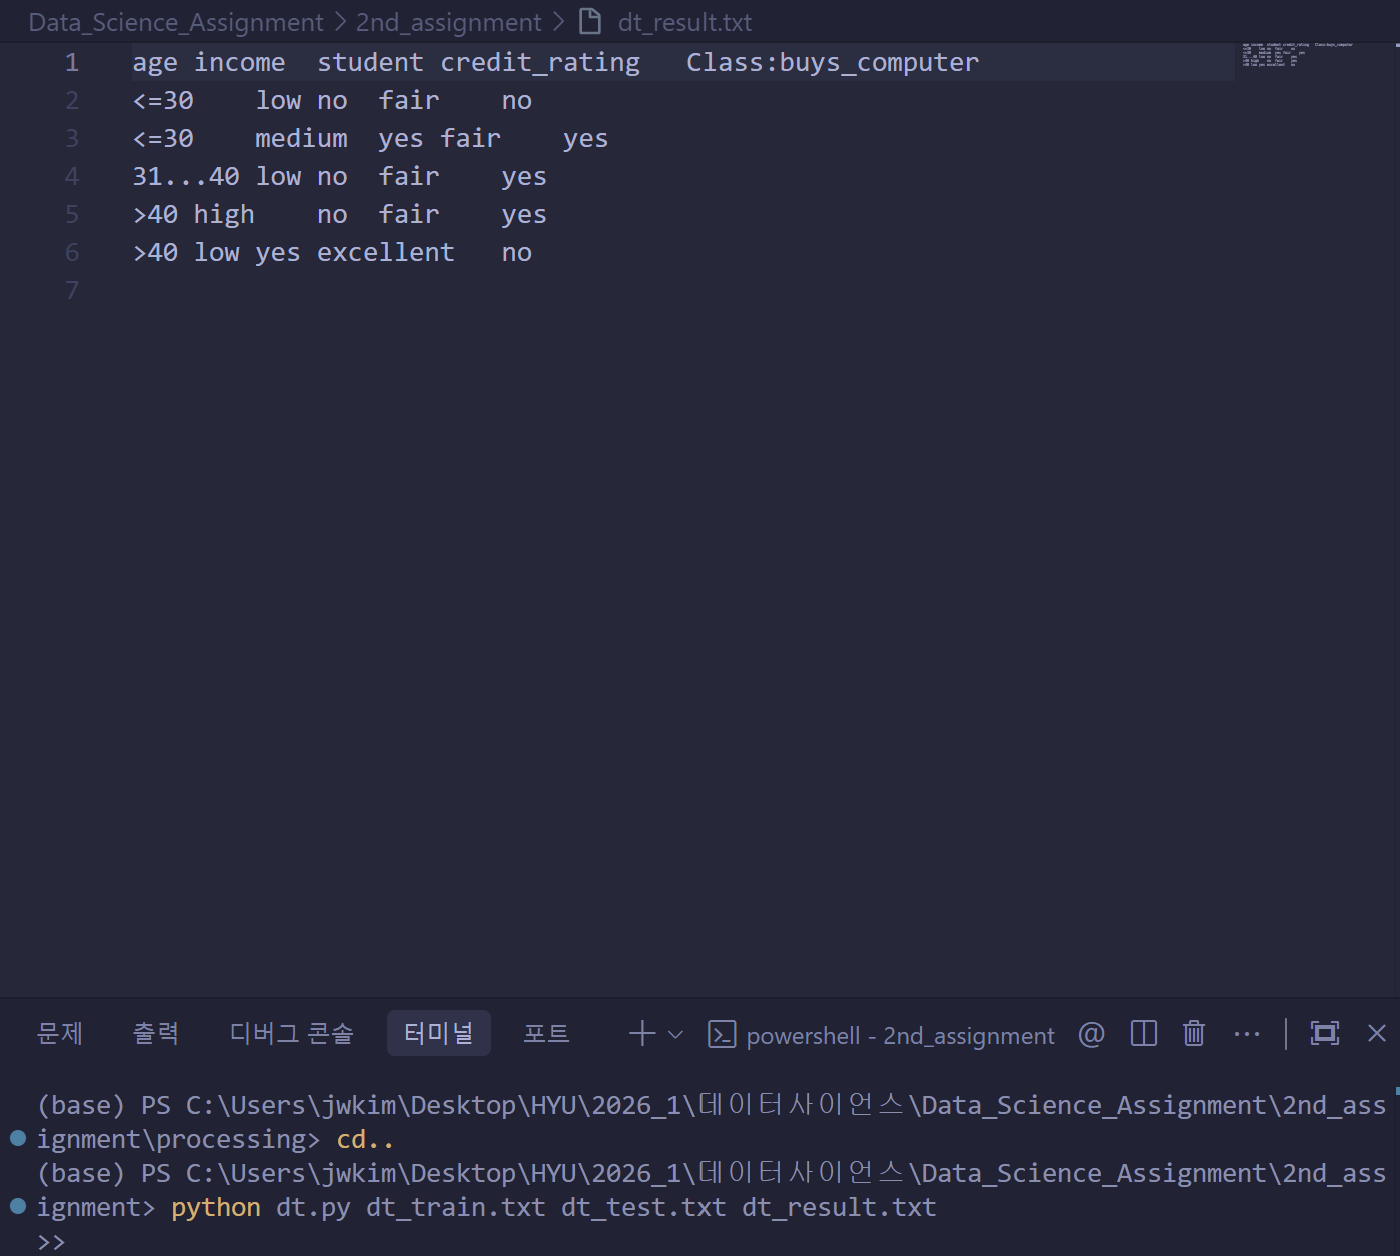
\includegraphics[width=0.9\textwidth]{screenshot.png}
    \caption{터미널에서 \texttt{python dt.py dt\_train.txt dt\_test.txt dt\_result.txt} 실행 및 결과 파일 생성 확인 화면}
\end{figure}


% ============================================================
\section{개발 과정 및 설계 결정 상세 기록}
% ============================================================

\subsection{데이터 접근 방식: 인덱스 $\to$ 이름}

초기에는 각 행의 속성에 \texttt{row[0]}, \texttt{row[2]}처럼 인덱스로 접근하는 방식을 고려하였다. 그러나 이는 데이터셋마다 속성 순서가 다를 경우 코드를 수정해야 하는 하드코딩 문제를 야기한다. 이를 해결하기 위해 \texttt{dict(zip(header, values))} 패턴을 도입, \textbf{속성 이름으로 값에 접근하는 방식}으로 전환하였다.

\begin{minted}{python}
# 변경 전 (인덱스 기반 -- 하드코딩)
age = row[0]
buying = row[1]

# 변경 후 (이름 기반 -- 범용)
age    = row['age']
buying = row['buying']
\end{minted}

이 변경 덕분에 \texttt{buys\_computer}와 \texttt{car\_evaluation}처럼 속성 구성이 전혀 다른 두 데이터셋을 \textbf{동일한 코드}로 처리하는 범용성을 확보하였다.


\subsection{연속형처럼 보이는 값의 처리: 임계값 계산 불필요}

\texttt{age} 속성의 \texttt{<=30}, \texttt{31...40}, \texttt{>40} 같은 값은 부등호와 숫자를 포함하지만, \textbf{이미 범주화된 문자열 그대로 취급}하면 된다. 컴퓨터 입장에서 이 값들은 \texttt{income}의 \texttt{high}, \texttt{low}와 완전히 동일한 고유 텍스트 카테고리이다.

따라서 임계값(Threshold) 계산이나 이분할(Binary Split) 로직은 불필요하며, 데이터에 존재하는 고유값의 종류대로 N-갈래 가지치기를 그대로 수행한다. 이는 코드 복잡도를 크게 낮추면서도 정확성을 유지하는 핵심 설계 결정이었다.


\subsection{트리 노드 표현: Node 클래스 $\to$ 중첩 딕셔너리}

처음에는 \texttt{Node} 클래스를 정의하여 \texttt{attribute}, \texttt{children}, \texttt{label} 등의 필드를 관리하는 방식을 고려하였다.

\begin{table}[h]
\centering
\begin{adjustbox}{max width=\textwidth}
\begin{tabular}{lll}
\toprule
\textbf{방식} & \textbf{장점} & \textbf{단점} \\
\midrule
\texttt{Node} 클래스 & 타입 명시적, 확장성 & 클래스 정의 및 보일러플레이트 코드 필요 \\
중첩 \texttt{dict}   & 클래스 정의 불필요, \texttt{print()}로 즉시 디버깅 가능 & 타입 암묵적 \\
\bottomrule
\end{tabular}
\end{adjustbox}
\caption{트리 노드 표현 방식 비교}
\end{table}

\noindent\textbf{결론: 중첩 딕셔너리 채택.} Python에서 \texttt{dict}는 키-값 쌍으로 계층 구조를 자연스럽게 표현하며, \texttt{isinstance(tree, dict)}로 내부 노드와 리프 노드를 타입으로 구분할 수 있다. 코드 간결성과 디버깅 편의성이 결정적이었다.


\subsection{분할 기준 비교 실험}

\textbf{정답 파일이 어떤 분할 기준으로 생성되었는지}에 따라 트리 구조가 달라질 수 있으므로, 4가지 전략을 비교 실험하였다.

\begin{table}[h]
\centering
\begin{adjustbox}{max width=\textwidth}
\begin{tabular}{lll}
\toprule
\textbf{전략} & \textbf{1차 기준} & \textbf{동점 해소} \\
\midrule
기존 (최종 채택) & Information Gain & Gain Ratio \\
실험 A           & Gain Ratio 단독  & --- \\
실험 B           & Gini Index 단독  & --- \\
실험 C           & Gain Ratio       & Gini Index \\
\bottomrule
\end{tabular}
\end{adjustbox}
\caption{분할 기준 비교 실험 전략}
\end{table}

\noindent 초기 실험에서 4가지 전략이 모두 동일한 결과(87.57\%)를 보여, 파일 저장이 제대로 반영되지 않은 것이 아닌가 하는 의심이 제기되었다. 이를 해소하기 위해 \textbf{단일 스크립트 내에서 4가지 전략 함수를 동시에 실행}하는 정밀 재검증을 수행하였다.

\begin{minted}{python}
for name, select_fn in [('IG+GR_tie',   s1), ('GR_only',     s2),
                         ('Gini_only',   s3), ('GR+Gini_tie', s4)]:
    tree = build_tree_custom(train, features, target, select_fn)
    preds = [predict_one(tree, row, default) for row in test]
    match = sum(1 for i in range(len(preds)) if preds[i] == answer[i])
    print(f'{name}: {match}/{len(preds)} = {match/len(preds)*100:.2f}%')
\end{minted}

\begin{verbatim}
IG+GR_tie:   303/346 = 87.57%
GR_only:     303/346 = 87.57%
Gini_only:   303/346 = 87.57%
GR+Gini_tie: 303/346 = 87.57%
\end{verbatim}

코드 변경이 정확히 반영된 상태에서도 4가지 전략이 완벽히 동일한 결과를 냄을 확인하였다.

\subsubsection*{원인 분석 및 결론}

\texttt{car\_evaluation} 데이터셋의 6개 속성(\texttt{buying}, \texttt{maint}, \texttt{doors}, \texttt{persons}, \texttt{lug\_boot}, \texttt{safety})은 모두 3\textasciitilde 4개의 매우 유사한 고유값 개수를 가진다. 고유값 개수가 균등하면 Split Information의 보정 효과가 거의 없으므로 $\mathrm{GainRatio} \approx \mathrm{IG}$가 성립하며, Gini Index도 엔트로피 기반 척도와 유사한 속성 순위를 매긴다. 결과적으로 \textbf{4가지 전략 모두 동일한 트리를 생성}하게 된다.

분할 기준의 차이가 의미를 가지려면, 속성 간 고유값 개수의 편차가 큰 데이터셋(예: 한 속성은 2개, 다른 속성은 20개의 고유값)이 필요하다. 본 데이터셋에서는 어떤 분할 기준을 써도 성능 차이가 없으므로, \textbf{가장 직관적인 Information Gain을 기본 기준으로 유지하되 Gain Ratio Tie-break를 보험용으로 탑재}하는 현재 설계를 그대로 최종 채택하였다.


% ============================================================
\section{테스트 결과}
% ============================================================

\subsection{소규모 데이터셋 (\texttt{buys\_computer})}

\begin{verbatim}
python dt.py dt_train.txt dt_test.txt dt_result.txt
\end{verbatim}

\begin{table}[h]
\centering
\begin{adjustbox}{max width=\textwidth}
\begin{tabular}{ll}
\toprule
\textbf{검증 항목} & \textbf{결과} \\
\midrule
학습 데이터                     & \texttt{dt\_train.txt} (14행, 4개 속성) \\
테스트 데이터                   & \texttt{dt\_test.txt} (5행) \\
\textbf{정확도}                 & \textbf{5/5 = 100\%} \cmark \\
정답 파일과 바이트 단위 일치    & \cmark \\
탭 구분 / 행 순서 유지          & \cmark \\
\bottomrule
\end{tabular}
\end{adjustbox}
\caption{소규모 데이터셋 테스트 결과}
\end{table}

\subsection{대규모 데이터셋 (\texttt{car\_evaluation})}

\begin{verbatim}
python dt.py dt_train1.txt dt_test1.txt dt_result1.txt
\end{verbatim}

\begin{table}[h]
\centering
\begin{adjustbox}{max width=\textwidth}
\begin{tabular}{ll}
\toprule
\textbf{검증 항목} & \textbf{결과} \\
\midrule
학습 데이터        & \texttt{dt\_train1.txt} (1,383행, 6개 속성) \\
테스트 데이터      & \texttt{dt\_test1.txt} (346행) \\
\textbf{정확도}    & \textbf{303/346 = 87.57\%} \\
불일치 건수        & 43건 \\
\bottomrule
\end{tabular}
\end{adjustbox}
\caption{대규모 데이터셋 테스트 결과}
\end{table}

43건의 불일치는 의사결정 나무의 오버피팅(Overfitting) 특성상 자연스러운 현상이다. 학습 데이터에 과적합된 트리는 테스트 데이터의 일부 패턴을 놓치며, 가지치기(Pruning) 없이 트리를 끝까지 성장시키는 본 구현의 특성이 이를 심화시킨다.

\subsection{범용성 검증}

\textbf{동일한 코드(\texttt{dt.py})} 하나로 \texttt{buys\_computer}와 \texttt{car\_evaluation} 두 데이터셋을 모두 정상 처리하였다. 속성 이름, 속성 개수, 클래스 라벨의 종류가 완전히 달라도 코드 수정 없이 동작함을 확인하였다 $\to$ \textbf{하드코딩 없는 범용 설계 검증 완료} \cmark.

\end{document}
